\section{Intra-Domain Results}\label{sec:intra_results}

As described in \autoref{sec:results_benchmarking}, the precision-recall
benchmark on a dataset consisting purely of sketches is meant to remove the
edge detection preprocessing steps as possible biases. The pipeline
configurations used are the global LUMA+MEAN variant
(\autoref{fig:pipeline_global_luma_mean}) with the L2 and COS distance measures
and the local LUMA+PMEAN and LUMA+PMEAN2 pipelines
(\autoref{fig:pipeline_local_luma_pmean}). Based on the results in
\autoref{sec:cross_results}, a grid cell number of $G=12$ and the cosine
distance measure are used for the global pipelines. The local LUMA+PMEAN and
LUMA+PMEAN2 variants are tested with $G=8$ and a patch size of $P=3$ in
combination with the histogram intersection distance metric $HI$. The size of
the codebooks remains at 1000 visual words. In all cases the Fast Discrete
Curvelet Transform uses the parameters $N_s=4$ and $N_{\theta}=12$.

As the graphs in \autoref{fig:results_precision} show, all four descriptors
exhibit a large variation of precision values across the different categories.
The mean average precision shows a small advantage of the global descriptors
with $MAP(Q_{MEAN+L2})=0.139$ and $MAP(Q_{MEAN+COS})=0.150$ over the local
variants with $MAP(Q_{PMEAN+HI})=0.129$ and $MAP(Q_{PMEAN2+HI})=0.120$
respectively.

\autoref{fig:results_average_precision} breaks the results down and displays
the average precision for each category. Here, it is apparent, that both global
and local descriptors deal well with some categories like "calculator", "pear"
or "donut", while the average precision values for the "parrot" and "door
handle" categories stay well below $0.1$. \autoref{fig:results_sketch_examples}
displays a few examples from two successful categories and two "difficult"
categories. This is in line with the observations made by the creators of the
benchmark dataset \autocite{eitz_how_2012}, that state that the images appear
to be of varying difficulty for computational classification. 

\begin{figure}[h!]
    \centering
    \subfloat[]{%
        \begin{tabular}{ccc}
            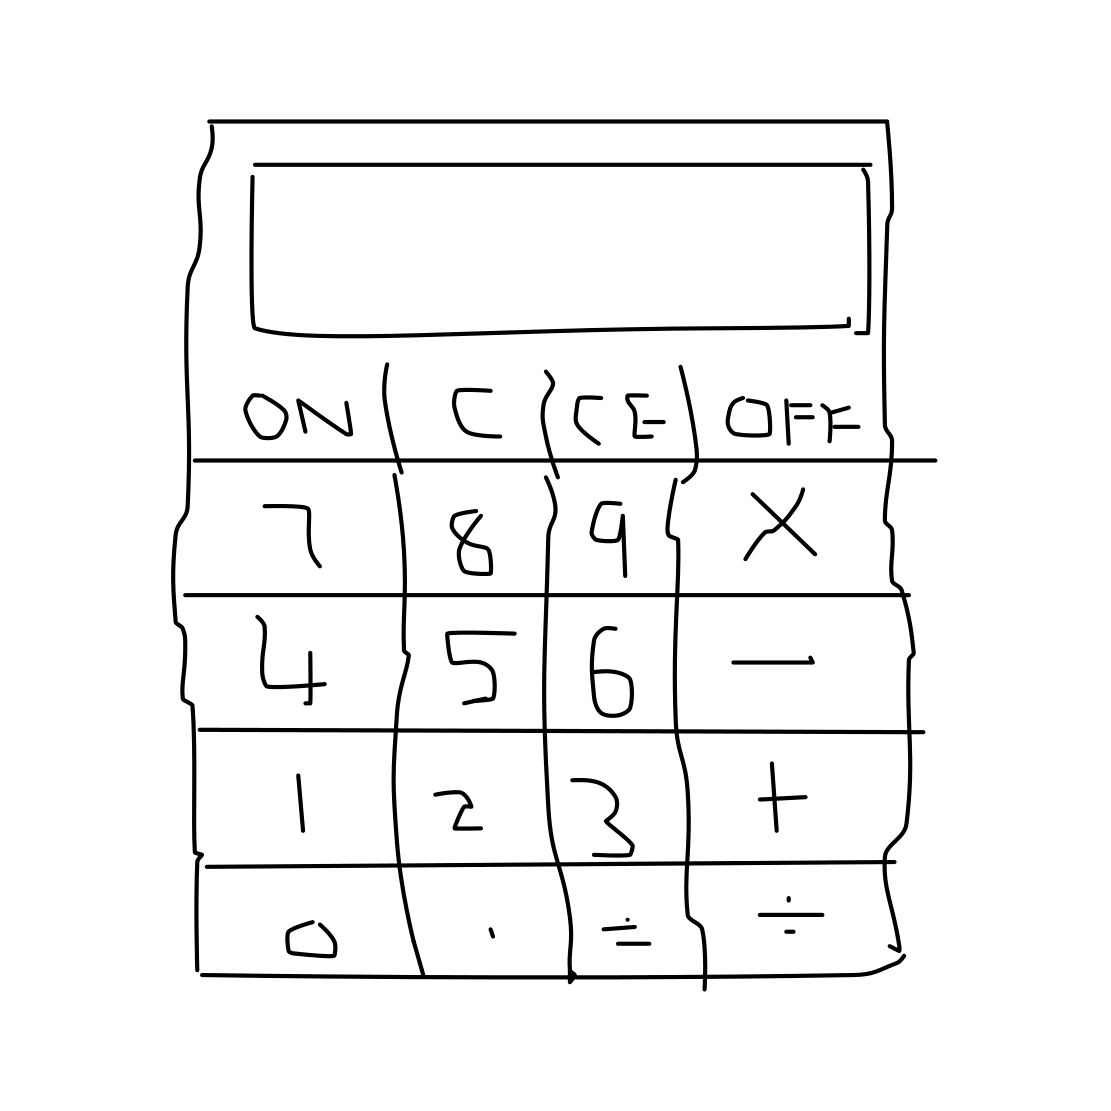
\includegraphics[width=0.15\textwidth]{illustrations/sketch_examples/calculator_1.png} &
            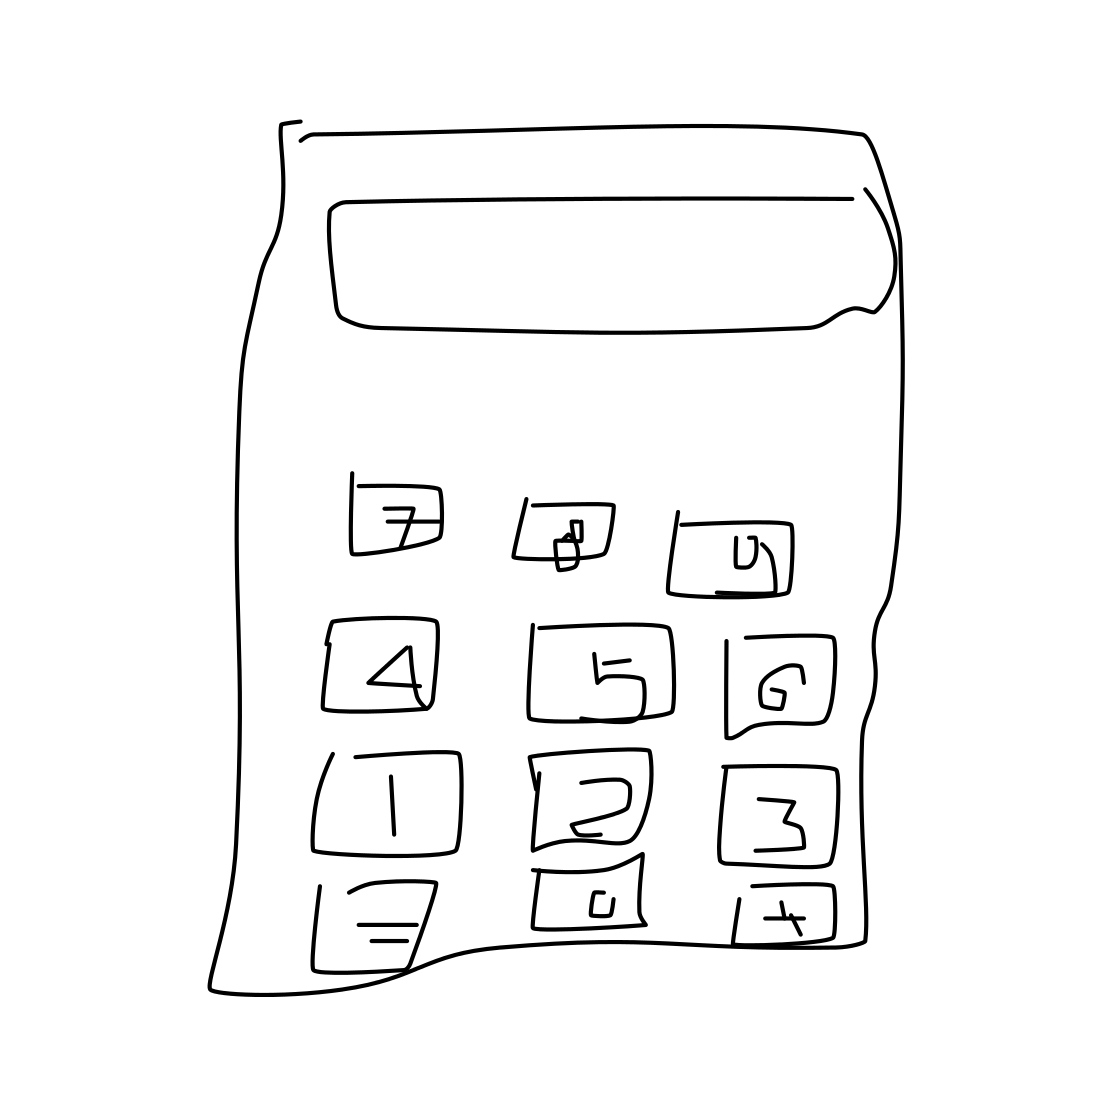
\includegraphics[width=0.15\textwidth]{illustrations/sketch_examples/calculator_2.png} &
            
\includegraphics[width=0.15\textwidth]{illustrations/sketch_examples/calculator_3.png} \\
            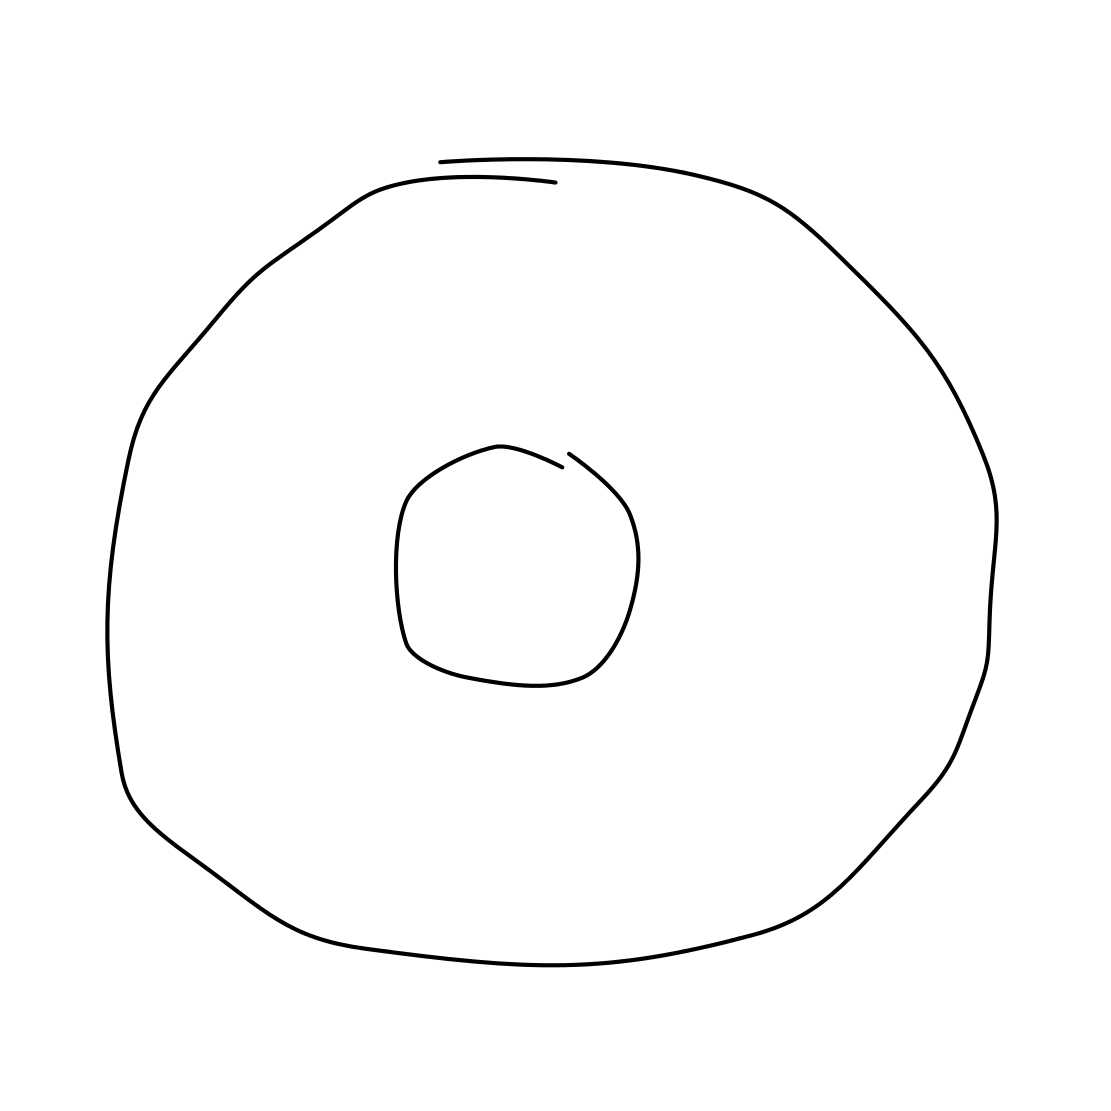
\includegraphics[width=0.15\textwidth]{illustrations/sketch_examples/donut_1.png} &
            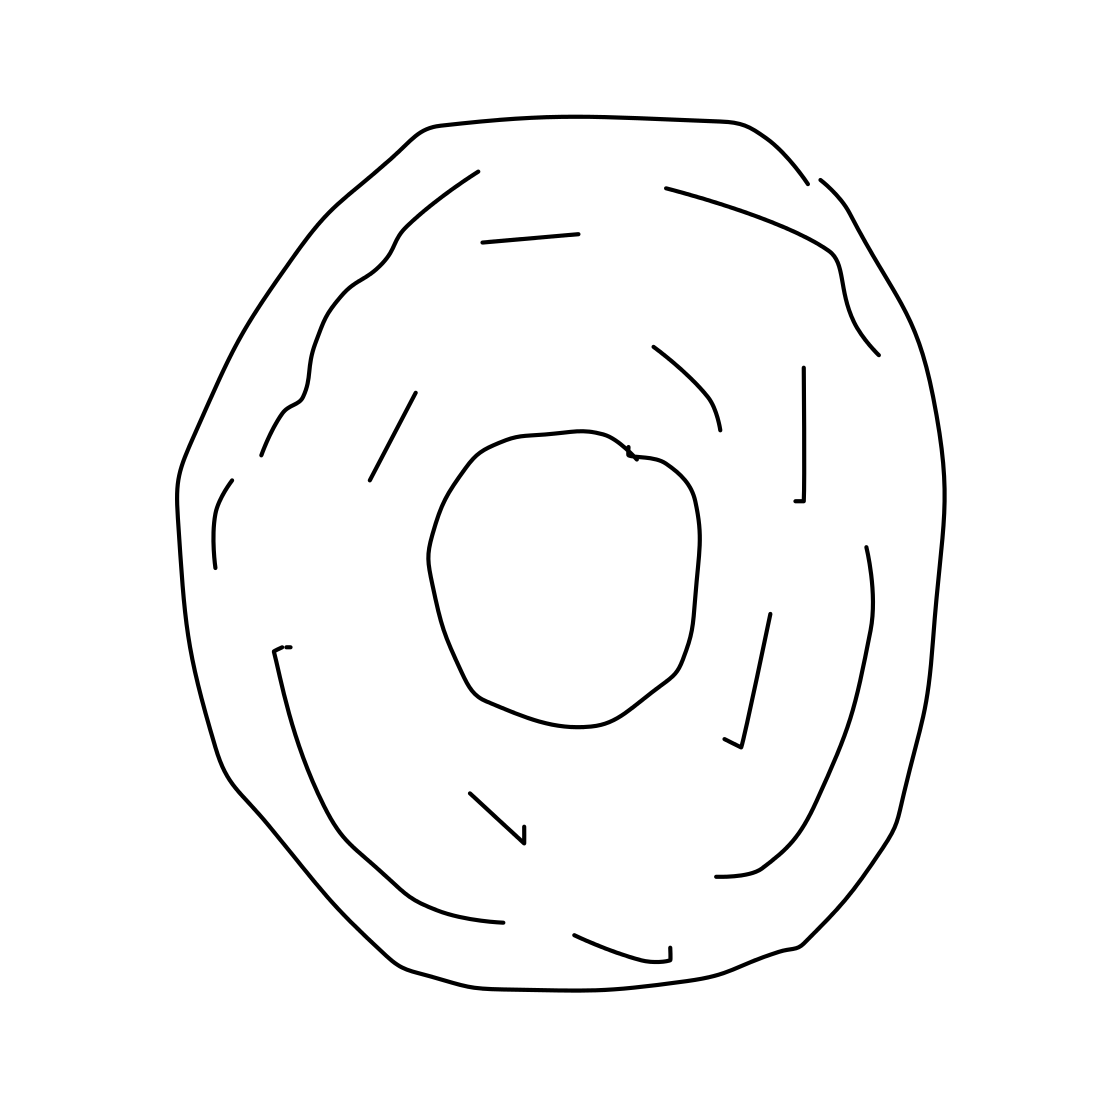
\includegraphics[width=0.15\textwidth]{illustrations/sketch_examples/donut_2.png} &
            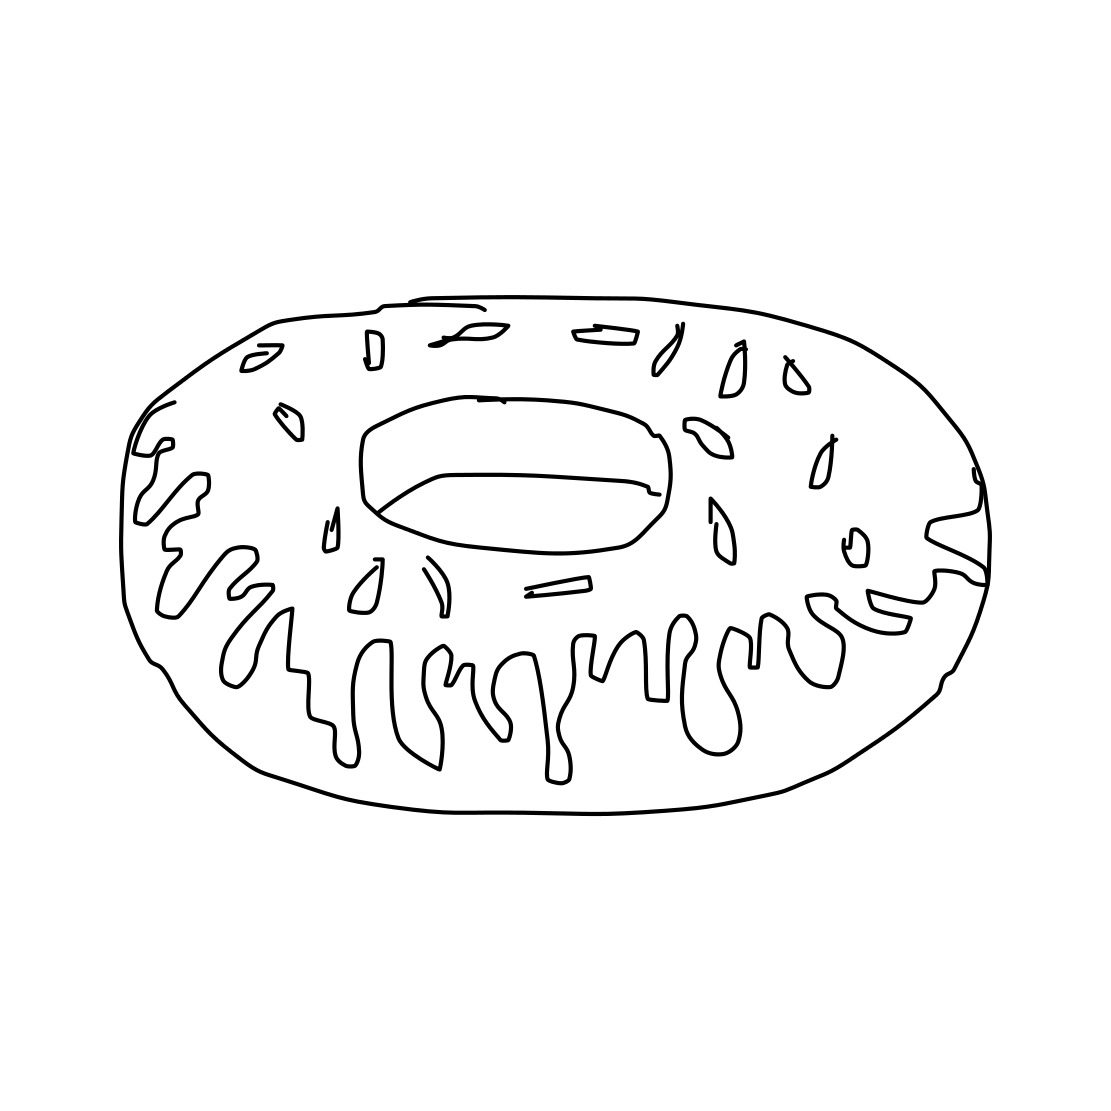
\includegraphics[width=0.15\textwidth]{illustrations/sketch_examples/donut_3.png}
        \end{tabular}
        \label{fig:results_sketch_examples_good}
    }
    \subfloat[]{%
        \begin{tabular}{ccc}
            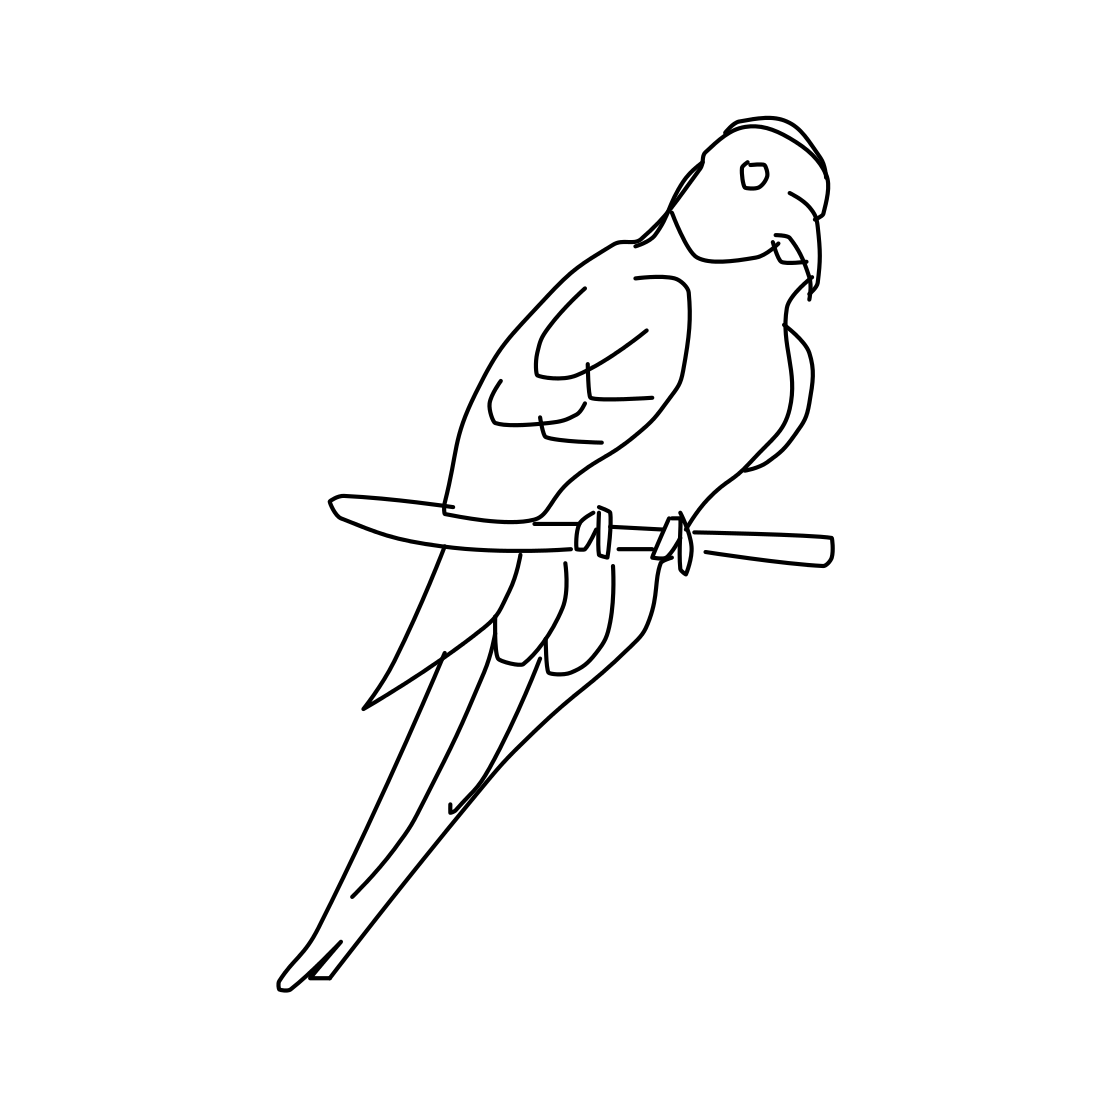
\includegraphics[width=0.15\textwidth]{illustrations/sketch_examples/parrot_1.png} &
            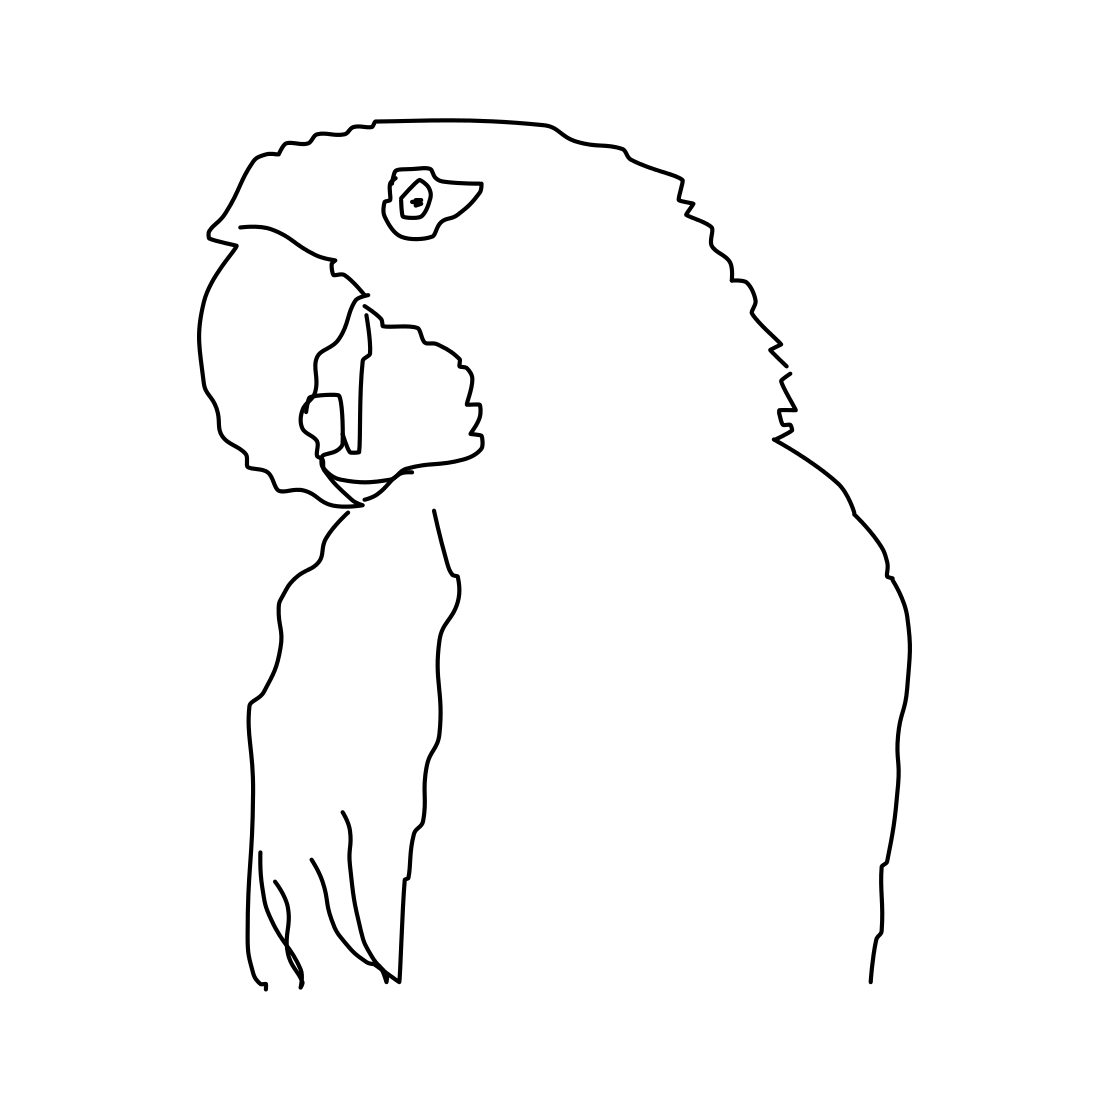
\includegraphics[width=0.15\textwidth]{illustrations/sketch_examples/parrot_2.png} &
            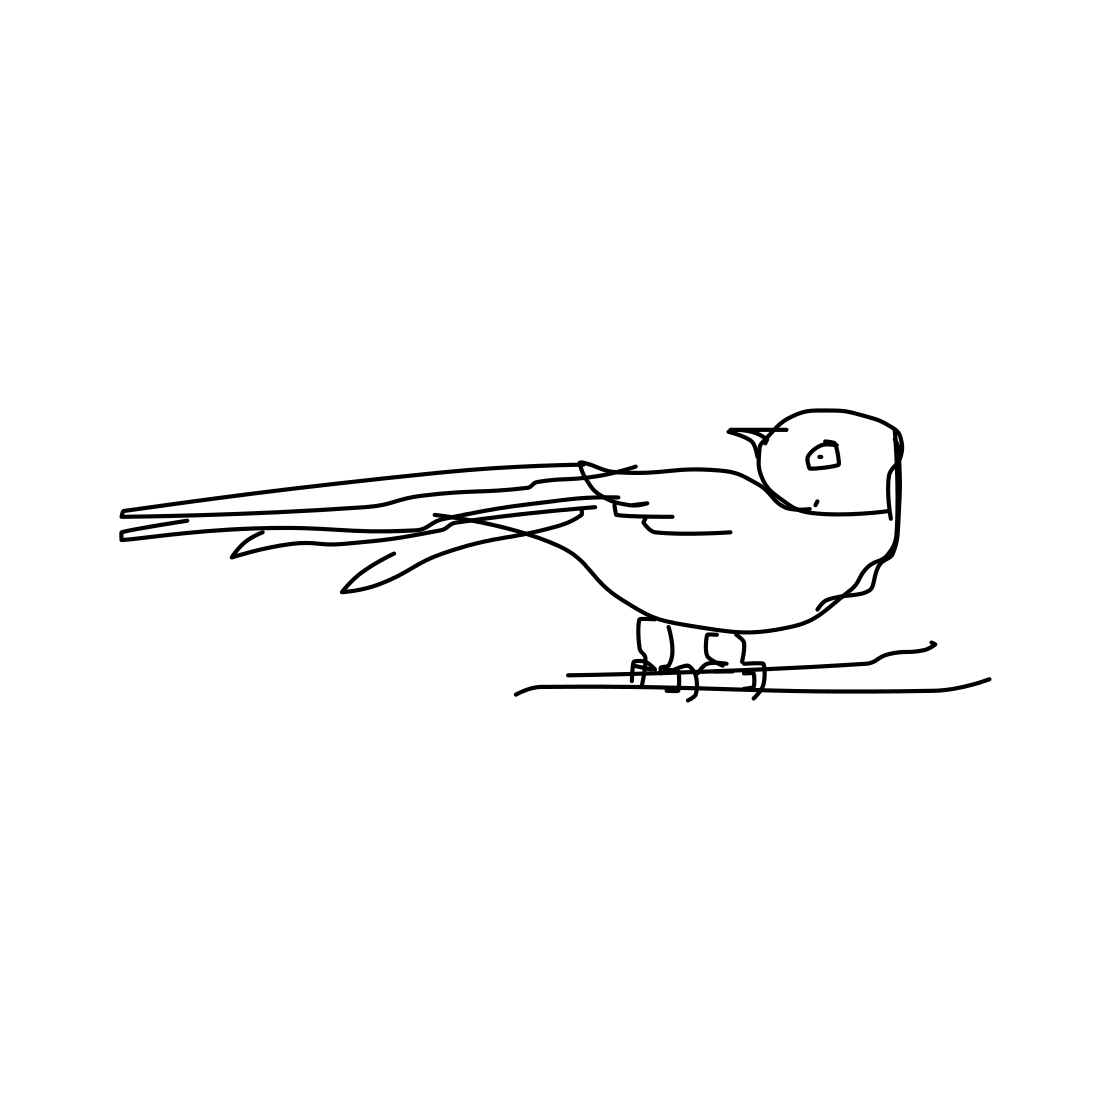
\includegraphics[width=0.15\textwidth]{illustrations/sketch_examples/parrot_3.png} \\
            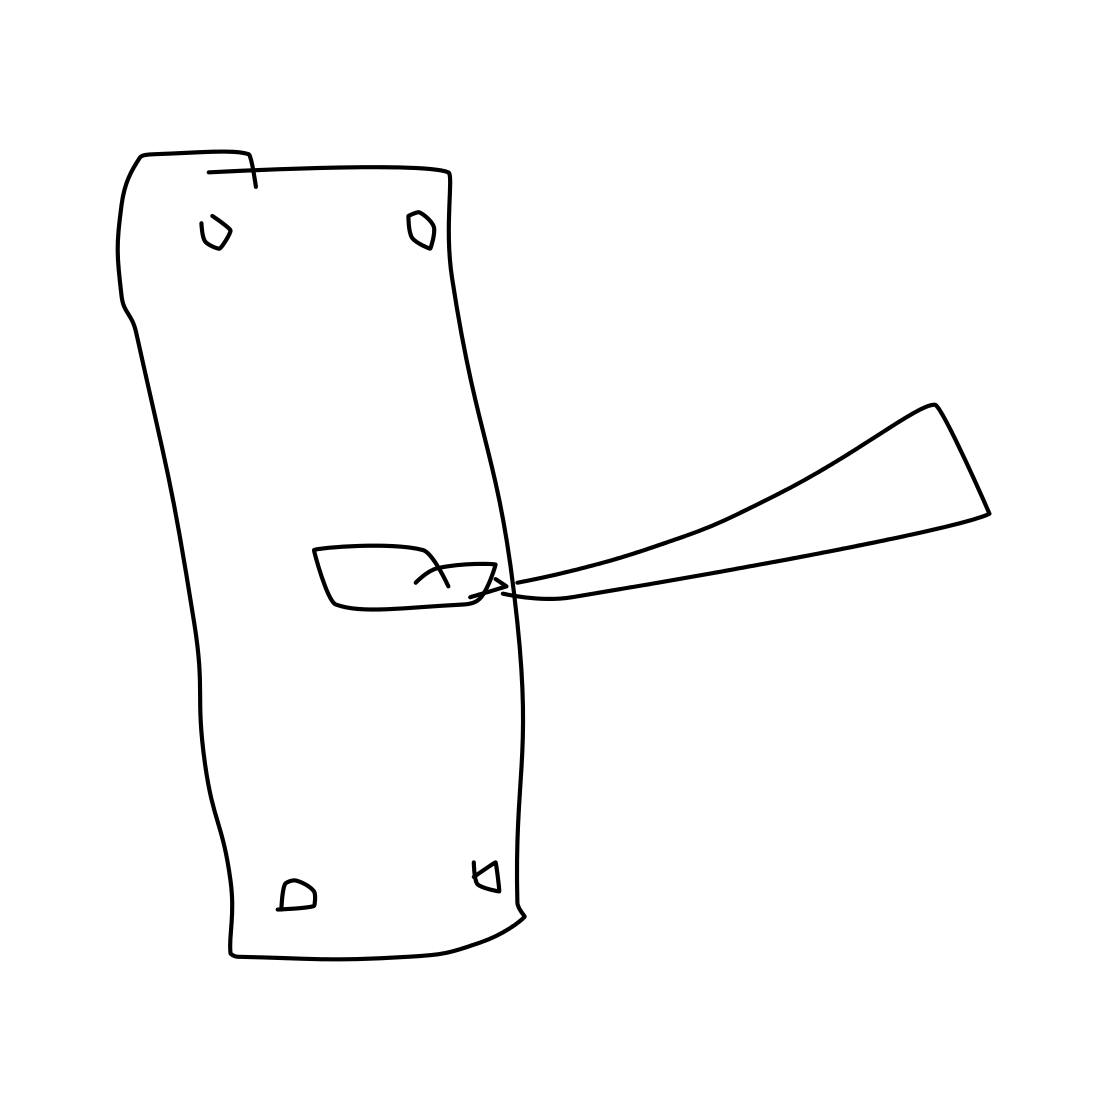
\includegraphics[width=0.15\textwidth]{illustrations/sketch_examples/doorhandle_1.png} &
            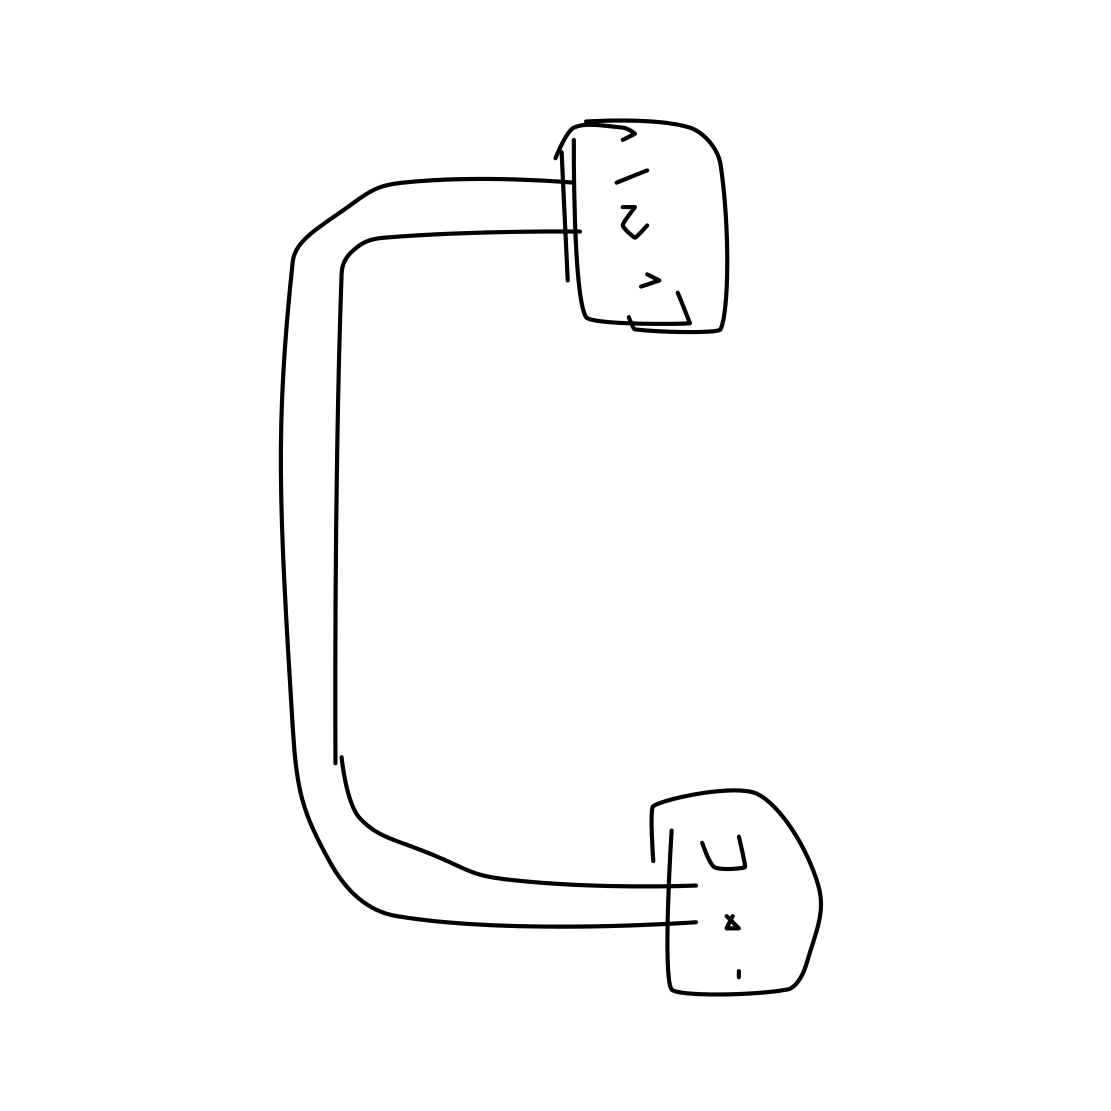
\includegraphics[width=0.15\textwidth]{illustrations/sketch_examples/doorhandle_2.png} &
            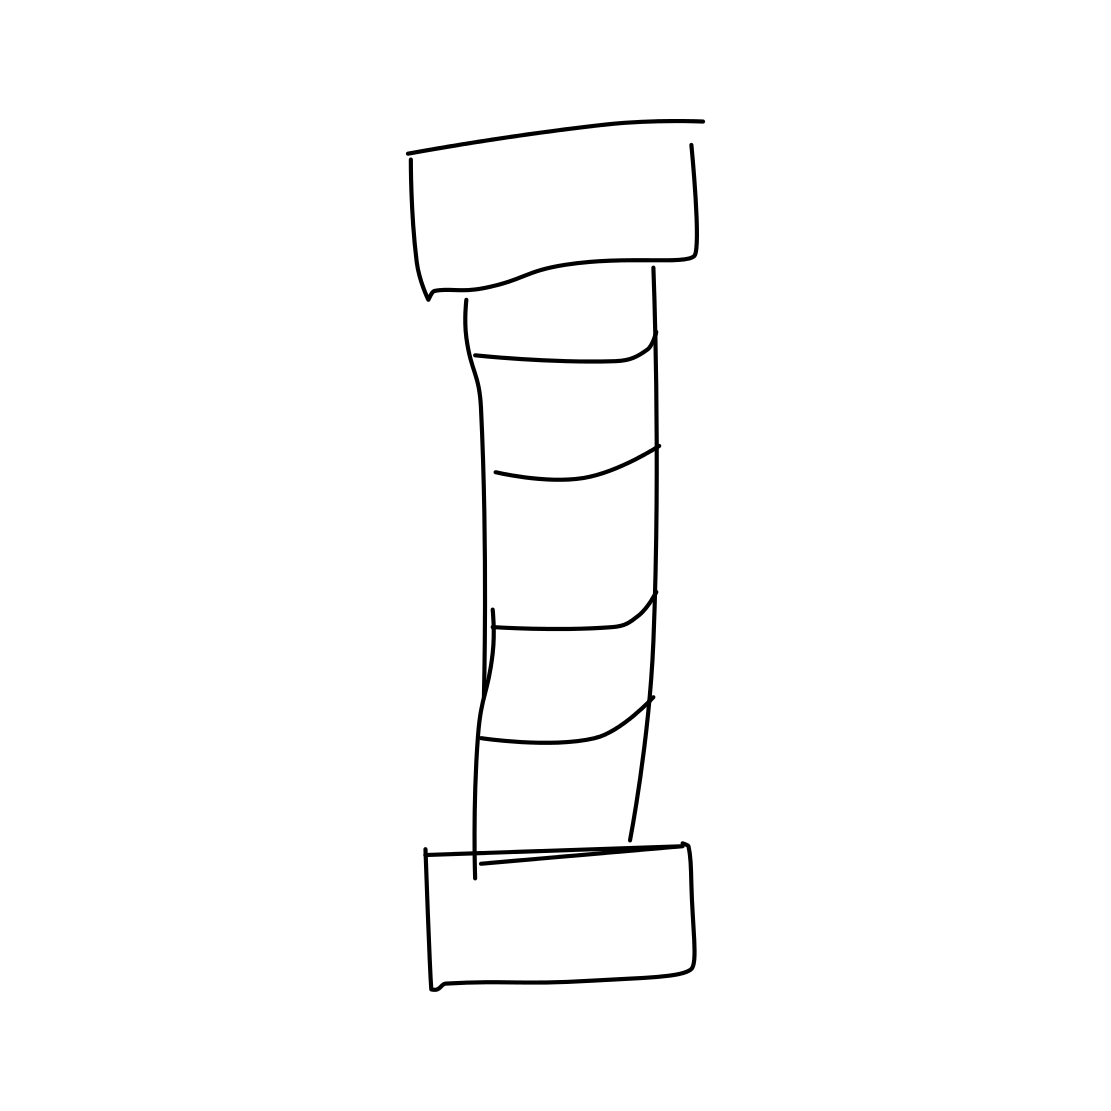
\includegraphics[width=0.15\textwidth]{illustrations/sketch_examples/doorhandle_3.png}
        \end{tabular}
        \label{fig:results_sketch_examples_bad}
    }
    \caption[Category Example Images]{
        The descriptors perform well on the categories "calculator" and "donut"
        \subref{fig:results_sketch_examples_good}, which exhibit a high degree
        of symmetry. The sketches from the categories "parrot" and "door
        handle" \subref{fig:results_sketch_examples_bad} do not have a uniform
        orientation or perspective or contain visually different
        representations of the object.
    }
    \label{fig:results_sketch_examples}
\end{figure}

\begin{figure}[h]
    \centering
    %\subfloat[Precisions for global LUMA+MEAN]{%
        %\pgfplotstableread[]{results/pr_g_luma_mean.csv}\resultsprglumamean
\begin{tikzpicture} %[trim axis left, trim axis right]
    \begin{axis}[
        small,
        no markers,
        xmin=0.1,
        xmax=1,
        ymin=0,
        xlabel=Recall,
        ylabel=Precision,
        legend entries={
            Mean,
            Category Skull,
            Category Pear,
            Category Squirrel
        },
        ymajorgrids,
        legend style={font=\tiny},
        legend pos=outer north east,
        cycle list name=exotic,
        ]
        \addplot+[draw=none, stack plots=y, no markers, forget plot] table[x=recall, y=min]{\resultsprglumamean};
        \addplot+[draw=none, stack plots=y, fill=gray!20, no markers, forget plot] table[x=recall, y expr=\thisrow{max}-\thisrow{min}]{\resultsprglumamean} \closedcycle;
        \addplot+[stack plots=false, thick] table[x=recall, y=precision]{\resultsprglumamean};
        \addlegendentryexpanded{Mean}
        \pgfplotsinvokeforeach{skull,pear,squirrel,cabinet,pumpkin,donut}{
            \addplot+ table[x=recall, y=#1]{\resultsprglumamean};
            \addlegendentryexpanded{Category "#1"}
        }

    \end{axis}
\end{tikzpicture}

        %\label{fig:results_precision_global_luma_mean}
    %}
    %\quad
    %\subfloat[Precisions for local LUMA+PMEAN]{%
        %\pgfplotstableread[]{results/pr_l_luma_pmean.csv}\resultsprllumapmean
\begin{tikzpicture} %[trim axis left, trim axis right]
    \begin{axis}[
        small,
        no markers,
        xmin=0.1,
        xmax=1,
        ymin=0,
        xlabel=Recall,
        ylabel=Precision,
        legend entries={
            Mean,
            Category Skull,
            Category Pear,
            Category Squirrel
        },
        ymajorgrids,
        legend style={font=\tiny},
        legend pos=outer north east,
        cycle list name=exotic,
        ]
        \addplot+[draw=none, stack plots=y, no markers, forget plot] table[x=recall, y=min]{\resultsprllumapmean};
        \addplot+[draw=none, stack plots=y, fill=gray!20, no markers, forget plot] table[x=recall, y expr=\thisrow{max}-\thisrow{min}]{\resultsprllumapmean} \closedcycle;
        \addplot+[stack plots=false, thick] table[x=recall, y=precision]{\resultsprllumapmean};
        \addlegendentryexpanded{Mean}
        \pgfplotsinvokeforeach{skull,pear,squirrel,cabinet,pumpkin,donut}{
            \addplot+ table[x=recall, y=#1]{\resultsprllumapmean};
            \addlegendentryexpanded{Category "#1"}
        }

    \end{axis}
\end{tikzpicture}

        %\label{fig:results_precision_local_luma_pmean}
    %}
    \newcommand{\plotpr}[1]{
    \addplot+[draw=none, stack plots=y, no markers, forget plot] table[x=recall, y=min]{#1};
    \addplot+[draw=none, stack plots=y, fill=gray!20, no markers, forget plot] table[x=recall, y expr=\thisrow{max}-\thisrow{min}]{#1} \closedcycle;
    \addplot+[stack plots=false, thick] table[x=recall, y=precision]{#1};
    \pgfplotsinvokeforeach{skull,pear,squirrel,cabinet,pumpkin,donut}{
        \addplot+ table[x=recall, y=##1]{#1};
    }
}

\pgfplotstableread[]{results/pr_g_luma_mean_l2.csv}\resultsprglumameaneucl
\pgfplotstableread[]{results/pr_g_luma_mean_cos.csv}\resultsprglumameancos
\pgfplotstableread[]{results/pr_l_luma_pmean.csv}\resultsprllumapmean
\pgfplotstableread[]{results/pr_l_luma_pmean2.csv}\resultsprllumapmeantwo
\begin{tikzpicture} %[trim axis left, trim axis right]
    \begin{groupplot}[
        group style={
            group size=2 by 2,
            group name=plots,
            xlabels at=edge bottom,
            ylabels at=edge left,
            vertical sep=1.5cm,
        },
        title style={
            font=\small,
        },
        name=mainplot,
        small,
        width=0.45\textwidth,
        no markers,
        xmin=0.1,
        xmax=1,
        ymin=0,
        xlabel=Recall,
        ylabel=Precision,
        ymajorgrids,
        legend columns=3,
        legend style={font=\tiny},
        legend cell align=left,
        cycle list name=exotic,
        ]
        \nextgroupplot[title=LUMA+MEAN+L2, legend to name=grouplegend]
            \plotpr{\resultsprglumameaneucl}
            \addlegendentryexpanded[black]{Mean}
            \pgfplotsinvokeforeach{skull,pear,squirrel,cabinet,pumpkin,donut}{
                \addlegendentryexpanded[black]{Category "#1"}
            }
        \nextgroupplot[title=LUMA+MEAN+COS]
            \plotpr{\resultsprglumameancos}
        \nextgroupplot[title=LUMA+PMEAN+HI]
            \plotpr{\resultsprllumapmean}
        \nextgroupplot[title=LUMA+PMEAN2+HI]
            \plotpr{\resultsprllumapmeantwo}
    \end{groupplot}
    \node[anchor=north] at ($(plots c1r2.outer south)!.5!(plots c2r2.outer south)$) {\ref{grouplegend}};
\end{tikzpicture}

    \caption[Precision and Recall Results]{
        The graphs show the results of applying the global LUMA+MEAN with the
        L2 and COS distance measures and the local LUMA+PMEAN and LUMA+PMEAN2
        pipelines to intra-domain retrieval of sketches. The areas indicate the
        overall spread of values across all categories while the line plots
        show results for selected categories.
    }
    \label{fig:results_precision}
\end{figure}

\begin{figure}[h]
    \centering
    \pgfplotstableread[]{results/ap_g_luma_mean_l2.csv}\resultsapglumameaneucl
\pgfplotstableread[]{results/ap_g_luma_mean_cos.csv}\resultsapglumameancos
\pgfplotstableread[]{results/ap_l_luma_pmean.csv}\resultsapllumapmean
\pgfplotstableread[]{results/ap_l_luma_pmean2.csv}\resultsapllumapmeantwo
\begin{tikzpicture} %[trim axis left, trim axis right]
    \begin{axis}[
        xbar=0.2pt,
        small,
        width=\textwidth,
        y=2.4ex,
        xmin=0,
        enlarge y limits={abs=1},
        xlabel={Average Precision},
        ylabel=Category,
        ylabel near ticks,
        xlabel near ticks,
        xtick={0,0.1,...,1},
        ytick=data,
        yticklabels from table={\resultsapglumameaneucl}{query},
        yticklabel style={
            font=\tiny,
        },
        xmajorgrids,
        legend entries={
            {global LUMA+MEAN+L2},
            {global LUMA+MEAN+COS},
            {local LUMA+PMEAN},
            {local LUMA+PMEAN2},
        },
        legend style={font=\tiny},
        %legend pos=outer north east,
        bar width=2pt,
        ]
        \addplot table[y expr=-\coordindex, x=average] {\resultsapglumameaneucl};
        \addplot table[y expr=-\coordindex, x=average] {\resultsapglumameancos};
        \addplot table[y expr=-\coordindex, x=average] {\resultsapllumapmean};
        \addplot table[y expr=-\coordindex, x=average] {\resultsapllumapmeantwo};
    \end{axis}
\end{tikzpicture}

    \caption[Average Precision by Category]{
        The average precision of the LUMA+MEAN, LUMA+PMEAN and LUMA+PMEAN2
        pipelines broken down by query category.
    }
    \label{fig:results_average_precision}
\end{figure}
\FloatBarrier
